\documentclass{article}
\usepackage[german]{babel}
\usepackage{float}
\usepackage{fourier}
\usepackage[utf8]{inputenc}
\usepackage[T1]{fontenc}
\usepackage{amsfonts,amsthm, amsmath}
\usepackage{listings}
% The following is needed in order to make the code compatible
% with both latex/dvips and pdflatex.
\ifx\pdftexversion\undefined
\usepackage[dvips]{graphicx}
\else
\usepackage[pdftex]{graphicx}
\DeclareGraphicsRule{*}{mps}{*}{}
\fi

\setlength\parindent{0pt}
\lstset{language=Erlang}

\begin{document}

\textbf{Team:} TEAM 01, Falco Winkler (FW), Daniel Schruhl (DS)\\
\\
\textbf{Aufgabenteilung:}
\begin{itemize}
    \item Starter (DS)
\end{itemize}

\textbf{Quellenangaben:}
\begin{itemize}
    \item Aufgabe 2, 25.04.2017, C.Klauck: \newline
    http://users.informatik.haw-hamburg.de/~klauck/VerteilteSysteme/aufg2.html
\end{itemize}

\textbf{Bearbeitungszeitraum:}
\begin{itemize}
	\item 13.04.2017 3h (FW)
	\item 24.04.2017 3h(DS)
	\item 25.04.2017(DS)
\end{itemize}

\textbf{Aktueller Stand:}
\begin{itemize}
	\item Starter-Modul fertig und getestet
	\item ggT-Modul angefangen
	\item Koordinator-Modul angefangen
\end{itemize}

\textbf{Änderung des Entwurfs:}
\begin{itemize}
    \item Keine Änderungen
\end{itemize}

\newpage

\section{Einführung und Ziele}
Mit dem Satz von Euklid ist es möglich, den größten gemeinsamen Teiler (ggT) zweier positiver ganzer Zahlen
($x,y \in \mathbb{Z}^{*}_{+}$) zu bestimmen (Gleichung \ref{equ:ggt-simple}).

Dabei wird der größte gemeinsame Teiler von $x$ und $y$ auf den größten gemeinsamen Teiler von $y$ und $\bmod{(x,y)}$
zurückgeführt.

\begin{equation}
\forall x,y \in \mathbb{Z}^{*}_{+}: ggT(x,y) = ggT(y,\bmod{(x,y)})
\label{equ:ggt-simple}
\end{equation}

Das erlaubt eine rekursive Berechnung des größten gemeinsamen Teilers.

Das Produkt soll diesen Algorithmus verteilt ausführen, verwalten und koordinieren, um den größten gemeinsamen Teiler zu
berechnen.

\subsection{Randbedingungen}
Um den ggT verteilt mit dem Algorithmus berechnen zu können, muss der Algorithmus angepasst werden
(Gleichung \ref{equ:ggt-distributed}). Das ermöglicht ein Terminieren in jedem ggT-Prozess mit dem ggT und nicht mit 0,
da bei $ggT(x,x)$ terminiert wird.

\begin{multline}
\forall x,y \in \mathbb{Z}^{*}_{+}: ggT(x,y) = ggT(y,\bmod{^{*}(x,y)})\\
\bmod{^{*}(x,y)} := \bmod{(x-1, y)} + 1
\label{equ:ggt-distributed}
\end{multline}

\subsection{Kontextbegrenzung}
Das System soll in Erlang umgesetzt werden. Es muss auf Computern mit Linux Betriebssystem lauffähig sein.

\newpage

\section{Gesamtsystem}

\subsection{Bausteinsicht}
\begin{figure}[H]
    \centering
    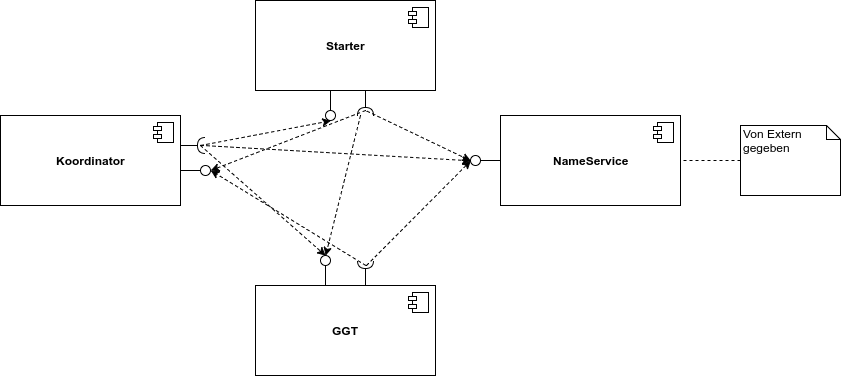
\includegraphics[width=1.0\textwidth]{component-diagram.png}
    \caption[seq-dia]{Komponentendiagramm der ggT-App}
    \label{fig:component-diagram}
\end{figure}

\subsection{Laufzeitsicht}

\newpage

\section{Subsysteme und Komponenten}

\subsection{Starter-Modul}
\subsubsection{Aufgabe und Verantwortung}
Der Starter steht zwischen Koordinator und ggT-Prozess. Er startet mehrere ggT-Prozesse mit den Initialisierungsdaten,
die vom Koordinator zur Verfügung gestellt werden (asynchron) und seinen konfigurierbaren Parametern.

\subsubsection{Schnittstelle}
\begin{lstlisting}
/* Nachricht zum Starten von ggT-Prozessen */
{steeringval,ArbeitsZeit,TermZeit,Quota,GGTProzessnummer}


/* Startet einen Starter Prozess */
start(StarterID): Integer -> PID
\end{lstlisting}
\{\textbf{steeringval},ArbeitsZeit,TermZeit,Quota,GGTProzessnummer\}:\\
Diese Schnittstelle wird für den Koordinator bereitgestelt und ermöglicht die Übergabe benötigter Konfigurationsparameter,
nach der Anfrage des Starters über getsteeringval.
Nach dem Ansprechen dieser Schittstelle sollte der Startvorgang der GGT Prozesse eingeleitet werden. Die ArbeitsZeit ist die simulierte Verzögerungszeit zur Berechnung in Sekunden, die TermZeit ist die
Wartezeit in Sekunden, bis eine Wahl für eine Terminierung initiiert wird, Quota ist die konkrete Anzahl an
benötigten Zustimmungen zu einer Terminierungsabstimmung und GGTProzessnummer ist die Anzahl der zu startenden
ggT-Prozesse.\\

\textbf{start(}StarterID\textbf{)}:\\
Startet den Starter mit der gegebenen eindeutigen Nummer.\\

\subsubsection{Entwurfsentscheidungen}
Der Starter ruft in seiner Initalisierungsphase an der Schnittstelle vom Koordinator seine benötigten Parameter zum
Starten von ggT-Prozessen asynchron ab. Zusätzlich werden noch die konfigurierbaren Parameter geladen. Mit diesen Daten
werden dann die ggT-Prozesse gestartet. Die Anzahl der zu startenden ggT-Prozesse wird durch die GGTProzessnummer in der
Schnittstelle definiert. Der Koordinator hält keine Referenz zu Starter - Prozessen, da nur die ggT Prozesse für Ihn
relevant sind.

\subsubsection{Konfigurationsparameter}
\begin{itemize}
    \item Praktikumsgruppe
    \item Teamnummer
    \item Nameservicenode definiert den Node des Nameservices
    \item Nameservicename definiert den Namen des registrierten Nameservices auf dem Nameservicenode
    \item Koordinatorname definiert den Namen des Koordinators
\end{itemize}

\newpage

\subsection{ggT-Modul}
\subsubsection{Aufgabe und Verantwortung}
TODO

\subsubsection{Schnittstelle}
\begin{lstlisting}
/* Einkommende Nachricht zum Setzen der Namen der Nachbarn */
{setneighbors,LeftN,RightN}

/* Einkommende Nachricht zum Setzen der von diesem Prozess */
/* zu berabeitenden Zahl fuer eine neue Berechnung */
{setpm,MiNeu}

/* Einkommende Nachricht zum Senden des rekursiven Aufrufes der ggT Berechnung */
{sendy,Y}

/* Einkommende Wahlnachricht fuer die Terminierung der aktuellen Berechnung */
{From,{vote,Initiator}}

/* Einkommende Erhaltenes Abstimmungsergebnis */
{voteYes,Name}

/* Einkommende Nachricht zum Senden des aktuellen Mis an From */
{From,tellmi}

/* Einkommende Nachricht zum Senden eines pongGGT an From */
{From,pingGGT}

/* Einkommende Nachricht zum Beenden des ggT-Prozesses */
kill

/* Funktion, die einen ggT-Prozess startet */
start(WorkingTime, TerminationTime, Quota, GGTName, Coordinator, NameService):
Integer X Integer X Integer X Atom X Tupel X PID -> PID
\end{lstlisting}
\{\textbf{setneighbors},LeftN,RightN\}: Setzt die Nachbarn. LeftN und RightN sind dabei Namen, die im NameService
(und lokal im Node) registriert sind.\\

\{From,\{\textbf{vote},Initiator\}\}: Wahlnachricht für die Terminierung der aktuellen Berechnung. Der Initiator ist der
Initiator dieser Wahl (Name des ggT-Prozesses, keine PID!) und From (ist PID) ist sein Absender.\\

\{\textbf{voteYes},Name\}: Erhaltenes Abstimmungsergebnis, wobei Name der Name des Absenders ist (keine PID!).\\

\{From,\textbf{tellmi}\}: Sendet das aktuelle Mi an From (ist PID): From ! \{mi,Mi\}. Wird vom Koordinator z.B. genutzt,
um bei einem Berechnungsstillstand die Mi-Situation im Ring anzuzeigen.\\

\{From,\textbf{pingGGT}\}: Sendet ein pongGGT an From (ist PID): From ! \{pongGGT,GGTname\}. Wird vom Koordinator z.B.
genutzt, um auf manuelle Anforderung hin die Lebendigkeit des Rings zu prüfen.\\


\textbf{start(}WorkingTime, TerminationTime, Quota, GGTName, Coordinator, NameService\textbf{)}: Startet einen
ggT-Prozess mit den gegebenen Parametern. Der GGTName setzt sich zusammen aus <PraktikumsgruppenID><TeamID><Nummer des ggT-Prozess><Nummer des Starters>.
Die WorkingTime beschreibt einen simulierten Arbeitsaufwand für die Berechnung und die TerminationTime beschreibt die
Zeit, nach der ein ggT-Prozess eine Terminierungsabstimmung durchführt. Die Quota ist die konkrete Anzahl an
notwendigen Zustimmungen zu einer Terminierungsabstimmung. Coordinator und NameService sind Referenzen für die
jeweiligen Dienste.\\

\subsubsection{Entwurfsentscheidungen}
Das Modul hält sich seinen State mit einer Config-Map. In dieser Map sind alle benötigten Variablen für den Algorithmus
und für den Betrieb des ggT-Moduls gespeichert.

\newpage

\subsection{Koordinator-Modul}
\subsubsection{Aufgabe und Verantwortung}

Der Koordinator verwaltet alle ggT Prozesse. Er kommuniziert mit Starter-Prozessen um diesen die benötigten
Werte zum Starten der ggT-Prozesse zu übergeben. Alle ggT-Prozesse müssen sich außerdem bei ihm anmelden,
und er übernimmt die Anordnung dieser in einem Ring, darüber hinaus die Terminierung des gesamten Systems auf Befehl eines
ggt-Prozesses.

Im Koordinator - Modul werden die drei Zustände durch drei receive - Schleifen realisiert. Alle Referenzen auf GGT
Prozesse werden in einer Erlang - Liste persistiert. Meldet sich ein GGT - Prozess beim Koordinator,
wird er am Ende dieser Liste angefügt.

Im Zustandsübergang zu "bereit" wird die Liste der GGT-Prozessnummern gemischt, iteriert,
und die Knoten bekommen ihre entsprechenden Nachbarn zugewiesen.


\subsubsection{Schnittstelle}

\subsubsection{Entwurfsentscheidungen}

\subsubsection{Konfigurationsparameter}

\end{document}